\section{Experimental Validation of SPNMF}
\label{sec:experiments}

In this section we conduct a set of experiments to assess the merits of the proposed method. We first perform a test on a synthetic signal to validate the model of SPNMF in section~\ref{SynthTest}. We then set-up the SPNMF to perform efficient source separation by quantifying the influence of the rank of factorization in section~\ref{setup:rank}, the effect of different divergences in section~\ref{setup:divergence} and finally the performance of the separation with different types of dictionaries in section~\ref{setup:dictionary}.


\subsection{Synthetic Tests}\label{SynthTest}

To illustrate how the SPNMF (Algorithm~\ref{AlgoMultipl}) works, we use a simple synthetic signal. The test signal models a mix of harmonic and percussive instruments. The harmonic part is simulated by a sum of sine waves that overlap in time and frequency. The first signal simulates a $C(3)$ with fundamental frequency $f_0 = 131$~Hz, the other one a $B(4)$ with $f_0 = 492$~Hz. To simulate the percussive part, we add $0.1$~s of Gaussian white noise for the first two second. For the last two seconds, we add $0.3$~s of Gaussian white noise filtered by a high-pass filter. The signal is $5$~s long and the sampling rate is $4000$~Hz. We compute the Short Time Fourier Transform (STFT) with a $512$ sample-long ($0.128$~s) Hann analysis window and a $50\%$ overlap. The spectrogram of the signal is represented in Figure~\ref{SpectroSynth}. As our input signal has four sources, we expect that one source can be represented by one component and therefore, a model of rank 4 ($k=4$) should adequately model the signals. More precisely, for the NMF and the PNMF we chose $k=4$ and for the SPNMF the rank of the harmonic part is $k_H=2$ and the rank of the percussive part is $k_P=2$. The choice of the rank of factorization is an important variable of the problem. In this case, we select it in order to illustrate the performance of the method. We will further discuss the importance of the choice of the rank of factorization in Section~\ref{setup:rank}. We compare the SPNMF with the PNMF and the NMF using the KL distance with multiplicative update rules as stated in~\cite{fevotte2009nonnegative}. The three algorithms are initialized with the same random positive matrices $W_{ini} \in \mathbb{R}^{n \times k}$  and $ H_{ini} \in \mathbb{R}^{k \times m}_{+} $.

The results of the decomposition are presented in Figure~\ref{resultONMF2}. The dictionary and activation matrices show the separation performance of the three methods. The NMF does not separate correctly the four components. By looking at the columns $2$ and $3$ of the dictionary matrix $W$ on Figure~\ref{resultONMF2}, the filtered Gaussian white noise and the $C(3)$ are separated in the same components which does not correspond to the expected result.
For the PNMF, the orthogonal components do not succeed to represent the two noises correctly. They are extracted in the same component and the total reconstruction error of the PNMF is high.
In this example, the SPNMF extracts the four components with the highest accuracy and performs better than the other methods. The two harmonic components are extracted in the orthogonal part (i.e., the columns $1$ and $2$ of the dictionary matrix) while the percussive components are extracted by the NMF part (columns $3$ and $4$). The SPNMF outperforms the two other methods and shows therefore the potential of the proposed algorithm for harmonic/percussive source separation.
%

\begin{figure}[t]

  \centering 
  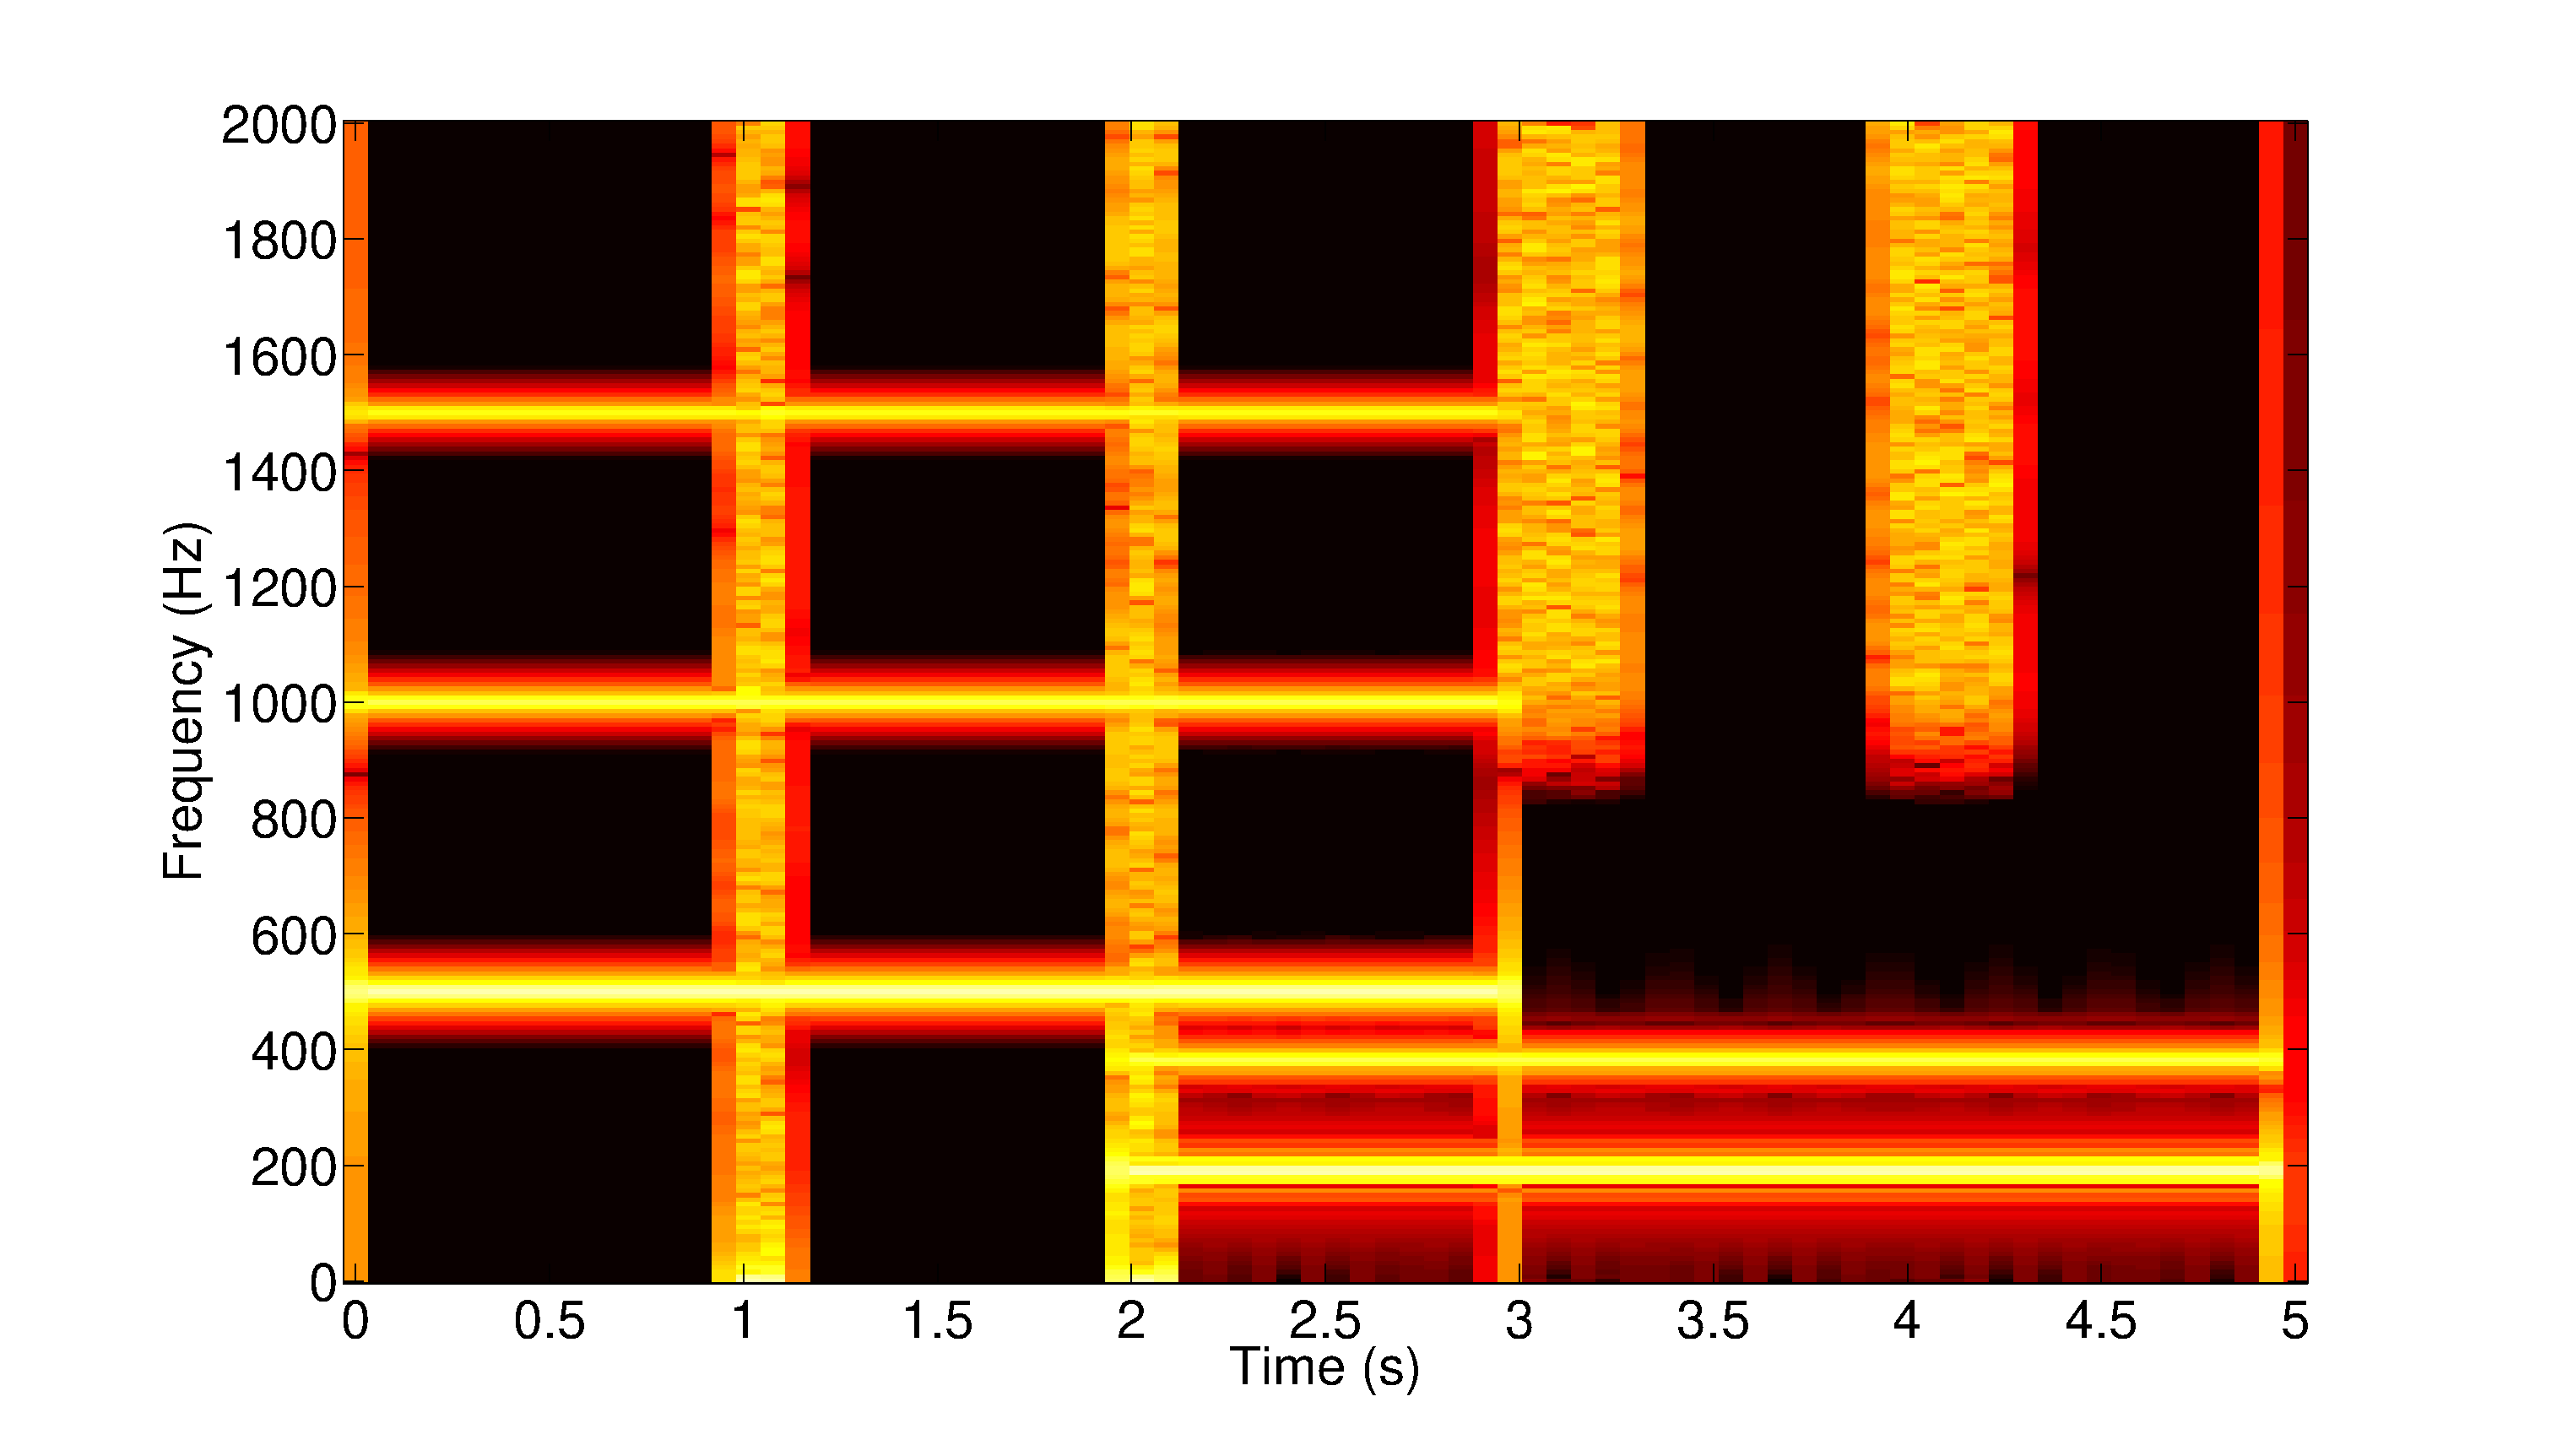
\includegraphics[width=9cm]{fig/synthetictestspectrogram}
%  \vspace{2.0cm}
  \caption{\label{SpectroSynth} Spectrogram of the synthetic test signal.}
  
\end{figure}

\begin{figure*}
   
	\centering    
  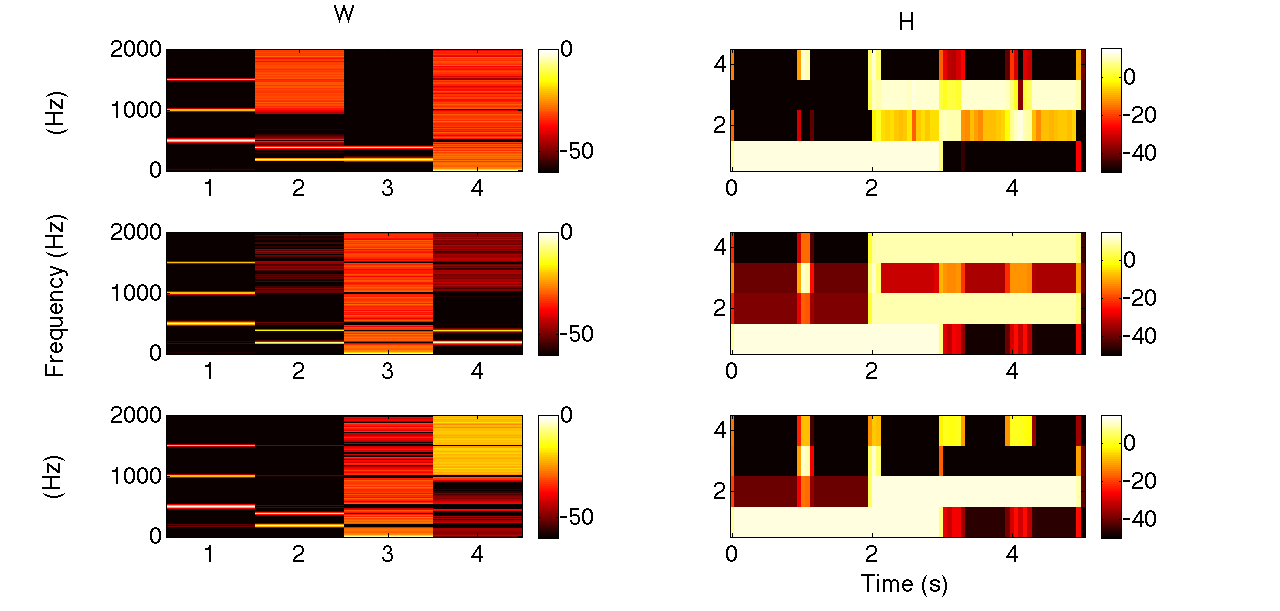
\includegraphics[width=15cm]{fig/WHcomp}

\caption{\label{resultONMF2} Results of the decomposition of the NMF (top matrices), PNMF (middle matrices) and SPNMF (bottom matrices).}


\end{figure*}


\subsection{Protocol and details of the test database}


To study the impact of using learned dictionaries in SPNMF (Algorithm \ref{AlgoDictionary}), we run several tests on the public SiSec database from \cite{SiSec10}. This database is composed of polyphonic real-world music excerpts. Each music signal contains percussive, harmonic instruments and vocals. It consists of four recordings whose durations range from $14$ to $24$~s. Our goal is to perform a harmonic/percussive decomposition. Thus, following~\cite{canadas2014percussive}, we do not consider the vocal part and we build mixture signals only from the percussive and harmonic instruments. All the signals are sampled at $44.1kHz$. We compute the STFT with a $1024$ and $2048$ sample-long Hann window with a $50\%$ overlap.
Three tests are run on these data:
\begin{enumerate}
	\item The first test aims at assessing the robustness of the SPNMF with respect to the rank of the PNMF part. 
	\item The second test is to evaluate which of the three divergences (Euc, KL and IS respectively) give the best harmonic/percussive decomposition results.
	\item The last test shows the influence of the dictionary on the separation performance. 
\end{enumerate} 
Note that the database we use for tuning the proposed method is different from the one in the evaluation phase in order to prevent any possible over-training. 
In order to evaluate and compare the results we then compute Signal to Distortion Ratio/Signal to Interference Ration/Signal to Artefact Ratio (SDR/SIR/SAR) that are common metrics for blind source separation with the BSS-Eval toolbox~\cite{bsseval}. 



\subsection{Comparison between PNMF and regularized NMF}

In this test the two methods are going to be tested using the same drum dictionary, with the same rank of factorization (the rank of factorization of the harmonic part is $k_H=150$) and the optimization is made with the KL divergence.
The SPNMF does not require further tuning. The two hyper parameters of the regularized method need to be optimised on a development database. This optimization process gives a set of value for the hyper parameters that maximise the average SDR SIR and SAR results, in our case we found that $k_{TSM} = 0.5$ and $k_{SSP}= 0.2$ where the most appropriate set of hyper parameters. However, it is not guaranteed that these fixed value maximise the score on each specific songs. 
Figure~\ref{regnmfcomp} show the results of the decomposition on the SiSec database. The results of the SPNMF for the SDR and SIR are above the regularized NMF.

These results shows that performance of the SPNMF over the RegNMF. The constraints can successfully replaced by a PNMF term in order to extract the harmonic instruments in order to simplify the optimization process. 


\begin{figure}[t]

  \centering 
  \includegraphics[width=9cm]{fig/RegNMFComp}
%  \vspace{2.0cm}
  \caption{\label{regnmfcomp} Comparaison of the SPNMF and the Regularized NMF on the SiSec database.}
  
\end{figure}


\subsection{Robustness wrt the rank of the harmonic part}
\label{setup:rank}

In the case where we use a fixed dictionary matrix, the only parameter of the algorithm is the rank of factorization of the harmonic part. In this experiment, we use the SPNMF algorithm with the fixed dictionary obtained from the STFT of a drum signal as described in Section~\ref{fixedict}. The algorithms are implemented using the multiplicative update rules from~\ref{euclidisteq},~\ref{KLdisteq} and~\ref{ISdisteq} and they all are  initialized with the same random non-negative matrices. 
We display the mean value of the separation results on Figure~\ref{RankOfFact}. When the rank of factorization is small, the Euclidean distance and the KL divergence do not give satisfying results. However, for $r>=100$, the results for both distances remain stable. With the IS divergence, the results seem independent of the rank of the factorization.

The optimization process of SPNMF is straightforward thanks to the robustness of the method wrt the rank of factorization. The number of components that can be decomposed by orthogonal basis functions is limited, and increasing the rank of factorization does not perturb the results as the harmonic part has to be orthogonal. For the rest of the article, the rank of factorization will be set to $r=100$ for all methods.



\begin{figure}[t]

  \centering 
  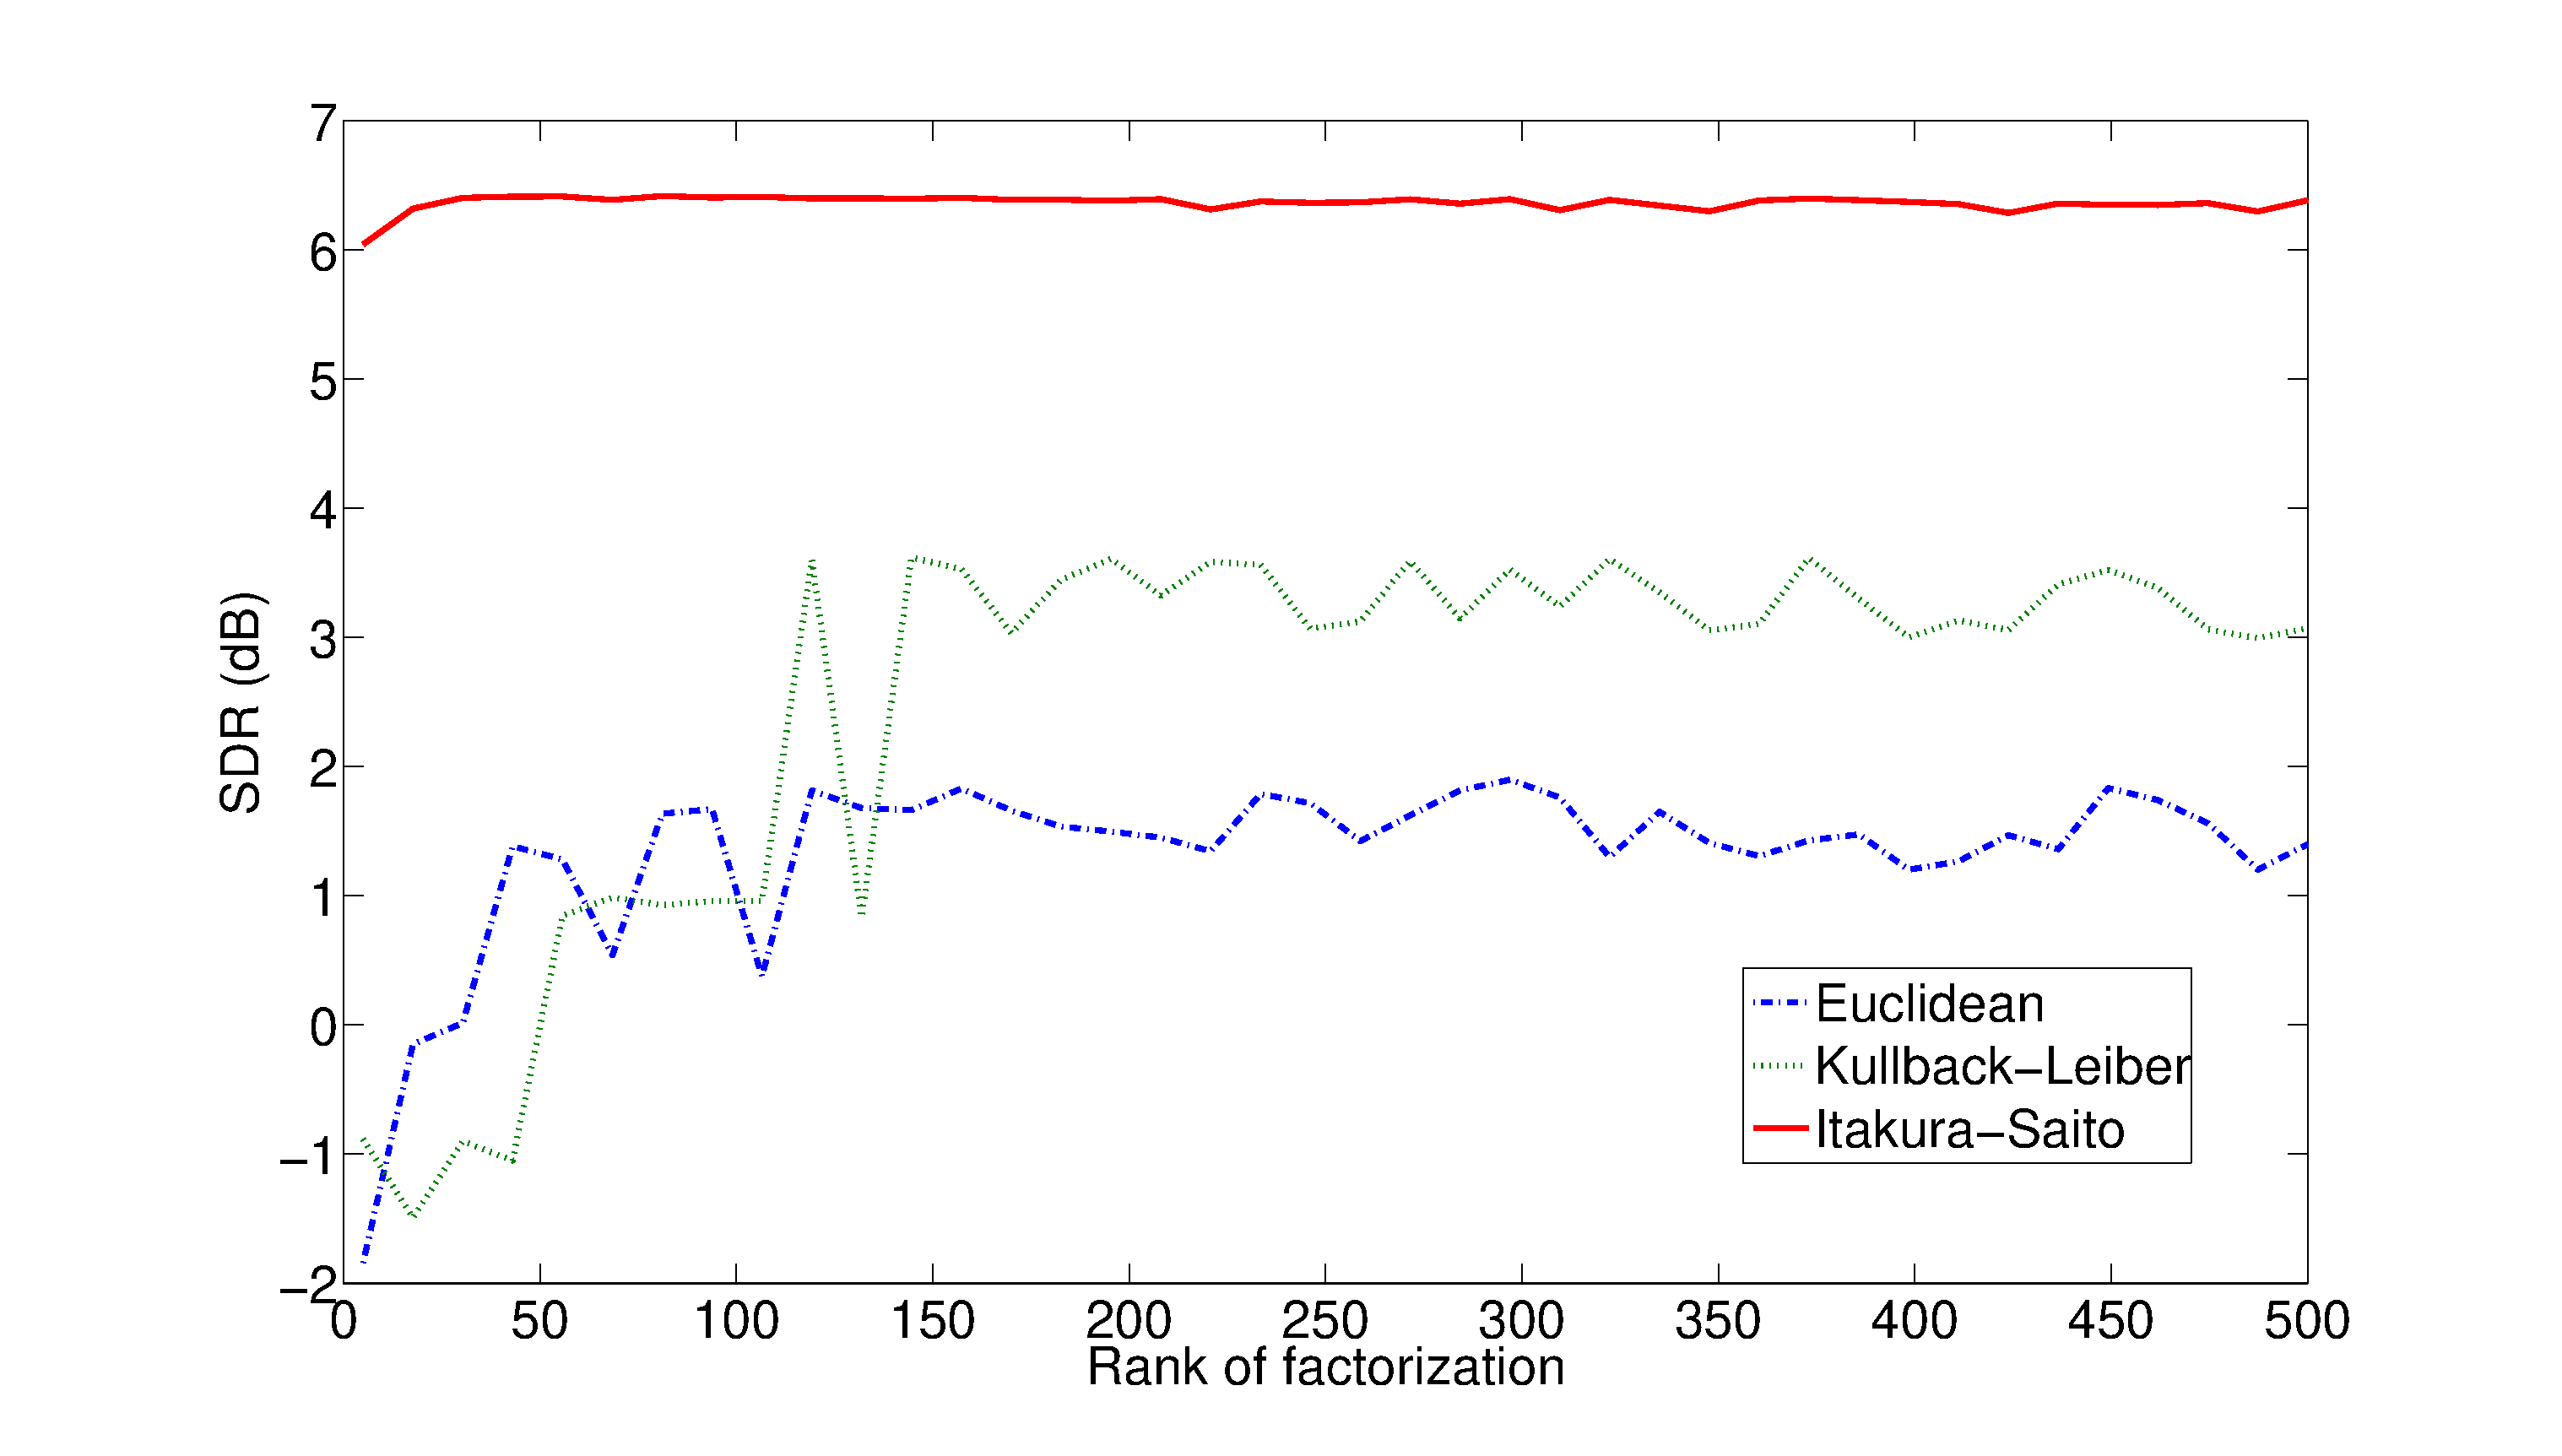
\includegraphics[width=9cm]{fig/RankOfFact}
%  \vspace{2.0cm}
  \caption{\label{RankOfFact} Optimization of the rank of factorization with the three divergences.}
  
\end{figure}




\subsection{Influence of the divergence}
\label{setup:divergence}

In this section we discuss the influence of the divergence in the results of the SPNMF algorithm. It has been established that the IS divergence is well suited for audio signal decomposition~\cite{gray1980distortion}, even if it does not always lead to superior separation performance~\cite{canadas2014percussive}. In this section, we perform a comparison of the three divergences on the SiSec database. Also, we compare two different window lengths ($1024$ samples and $2048$ samples) for the Fourier transform as it showed interesting results. We display on Figures~\ref{frame1024} and~\ref{frame2048} the mean of the results of the three algorithms computed on the SiSec database. Each box-plot is made up of a central line indicating the median of the data, upper and lower box edges indicating the $1^{st}$ and $3^{rd}$ quartiles while the whiskers indicate the minimum and maximum values. 

When the analysis window length is small, the percussive instruments are well represented and the energy is localized. Using a longer window spreads the percussive energy while the tonal components are well separated in the TF domain.

When the window size is small, Figure~\ref{frame1024} shows that the percussive decomposition is better for the Euclidean distance and the KL divergences. However, the harmonic components are not well separated in the TF domain and the orthogonal part of SPNMF does not perform a good separation.  
In the case of a long window, Figure~\ref{frame2048} shows that the IS divergence works better than the other divergences. The orthogonal part is more effective to extract the harmonic components as the finer frequency resolution allows for a better separation in the TF domain. The IS divergence is scale invariant. It means that the low energy components of the spectrogram bear the same relative importance as the higher ones which allows a good extraction of the percussive instruments even if the energy is spread temporally.


For the rest of the article, we will use the SPNMF algorithm with the IS divergence and a window size of 2048 samples for the STFT.


\begin{figure}[t]

  \centering 
  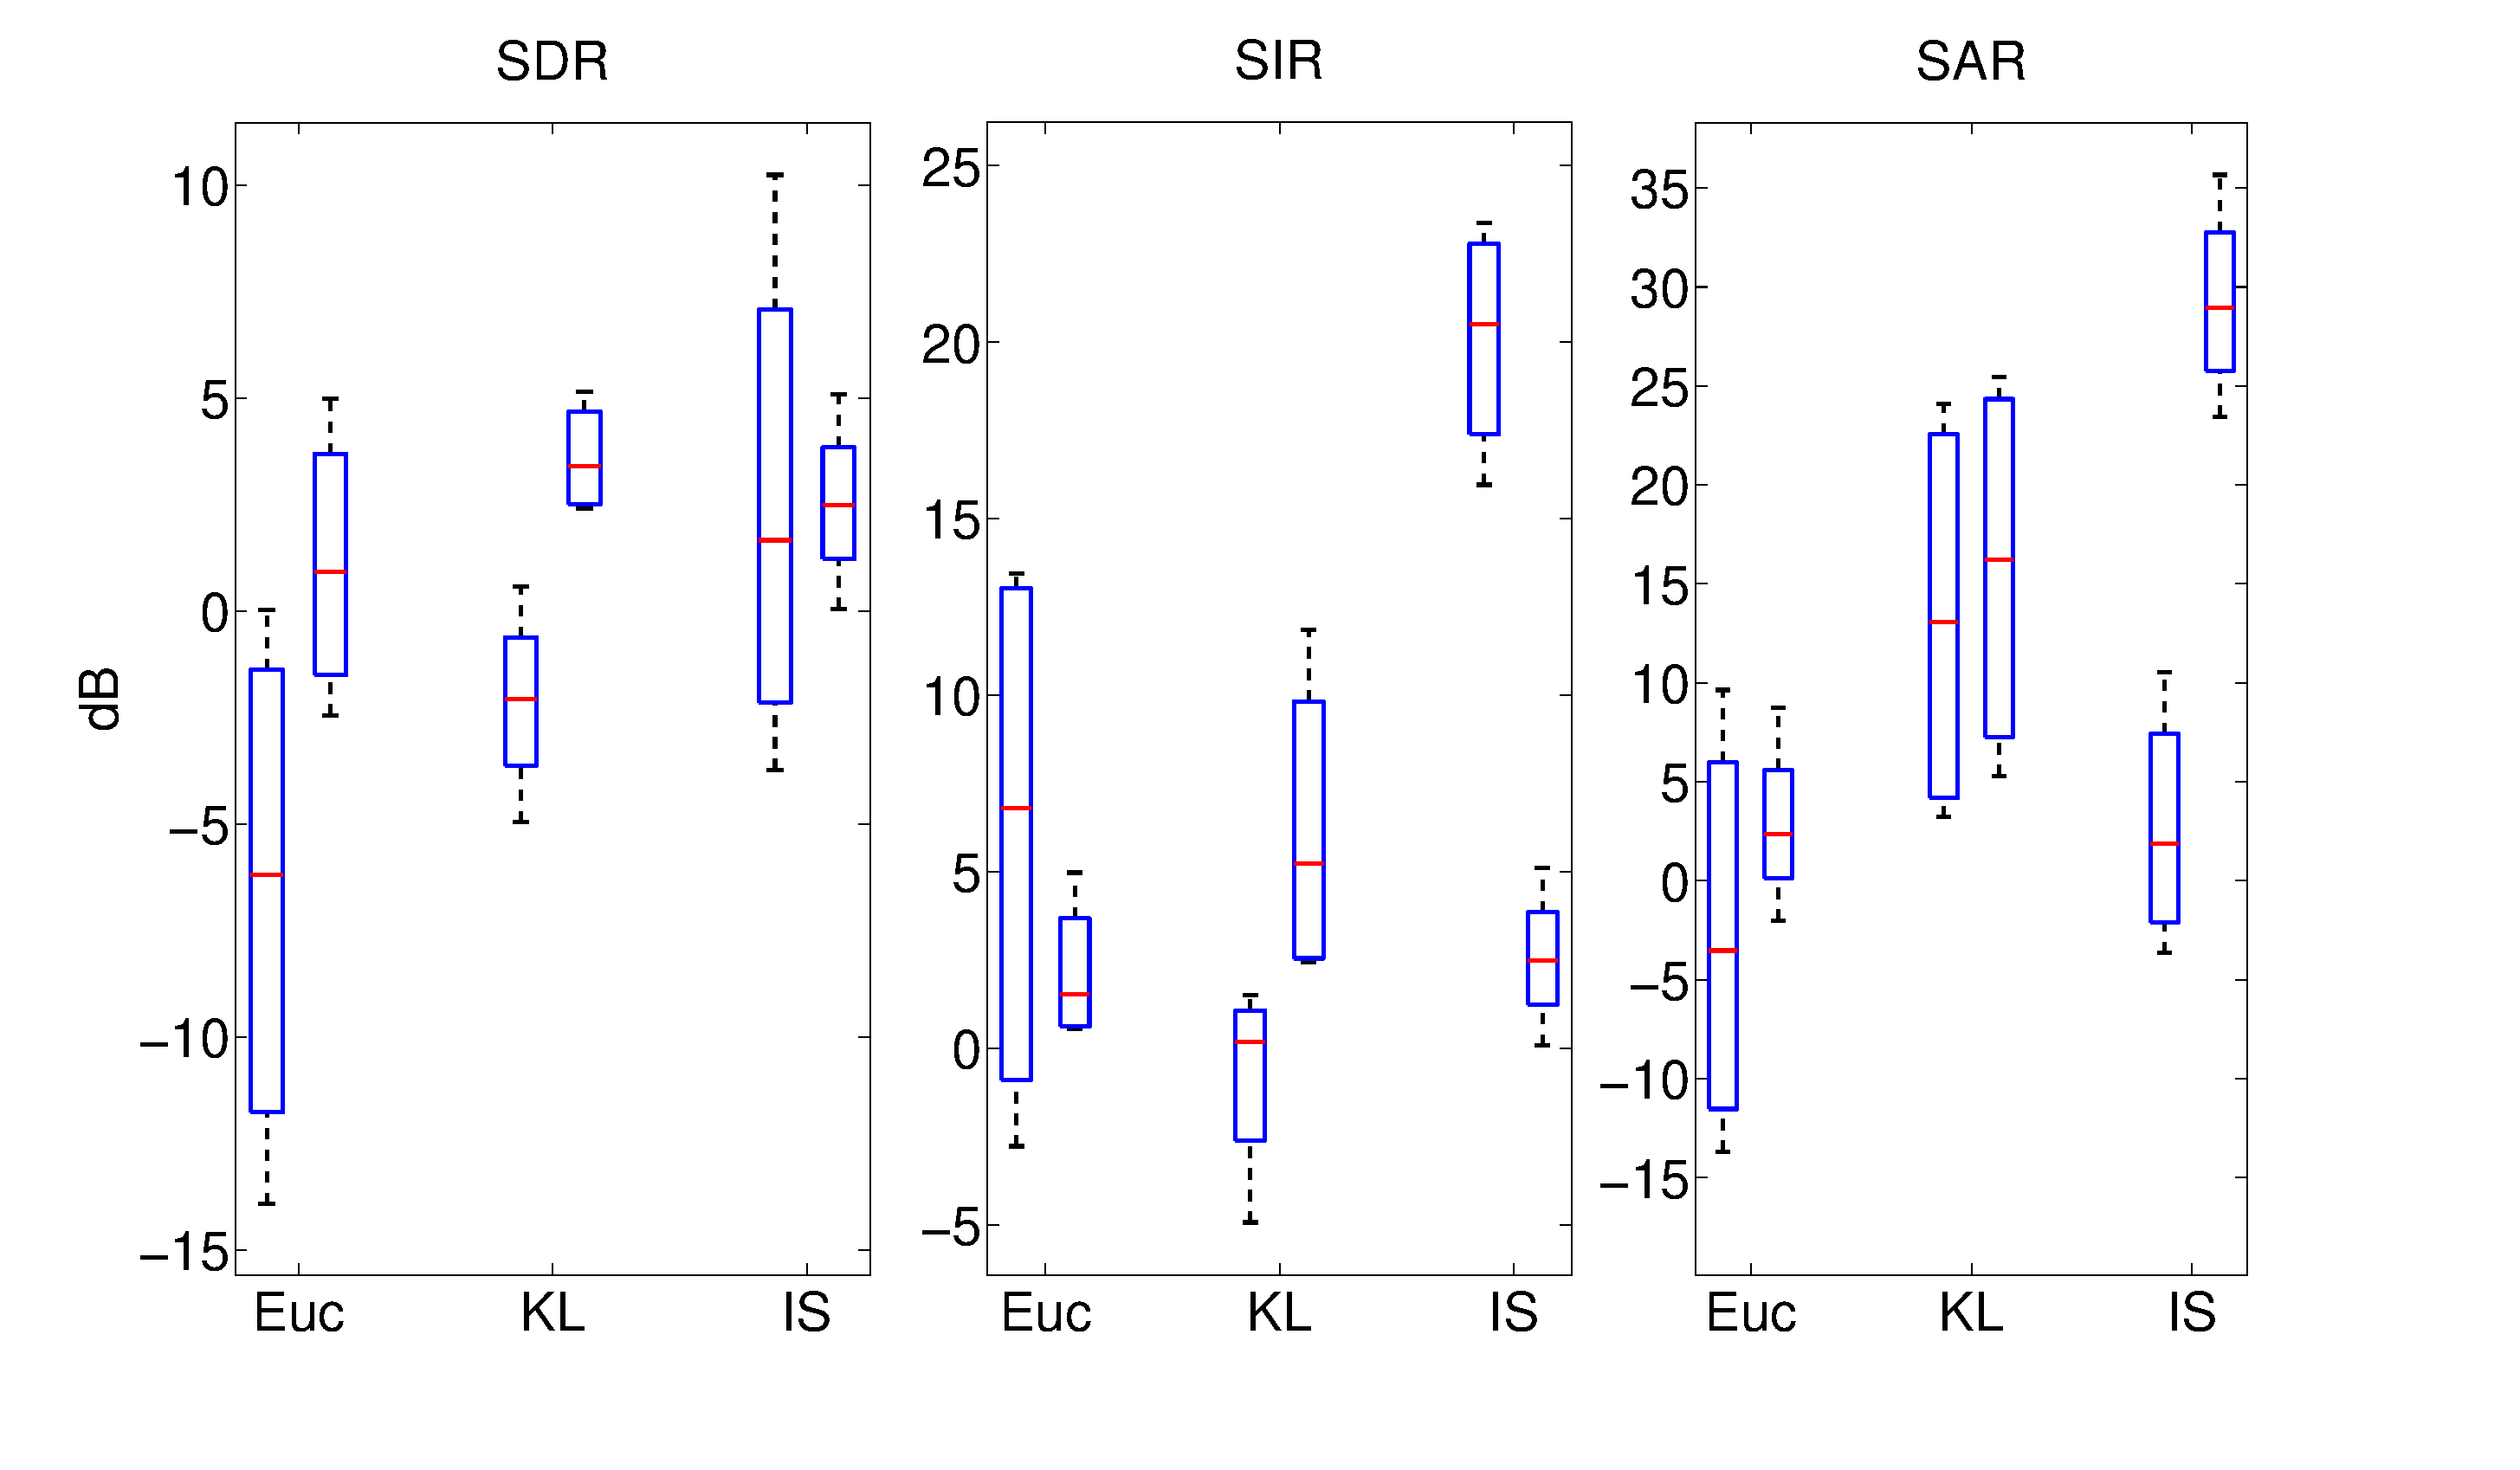
\includegraphics[width=9cm]{fig/NewDictDivTest1024}
%  \vspace{2.0cm}
  \caption{\label{frame1024} SDR, SIR and SAR of harmonic (left bar)/percussive (right bar) estimated sources on the SiSec database with a window frame of $1024$ samples.}
  
\end{figure}


\begin{figure}[t]

  \centering 
  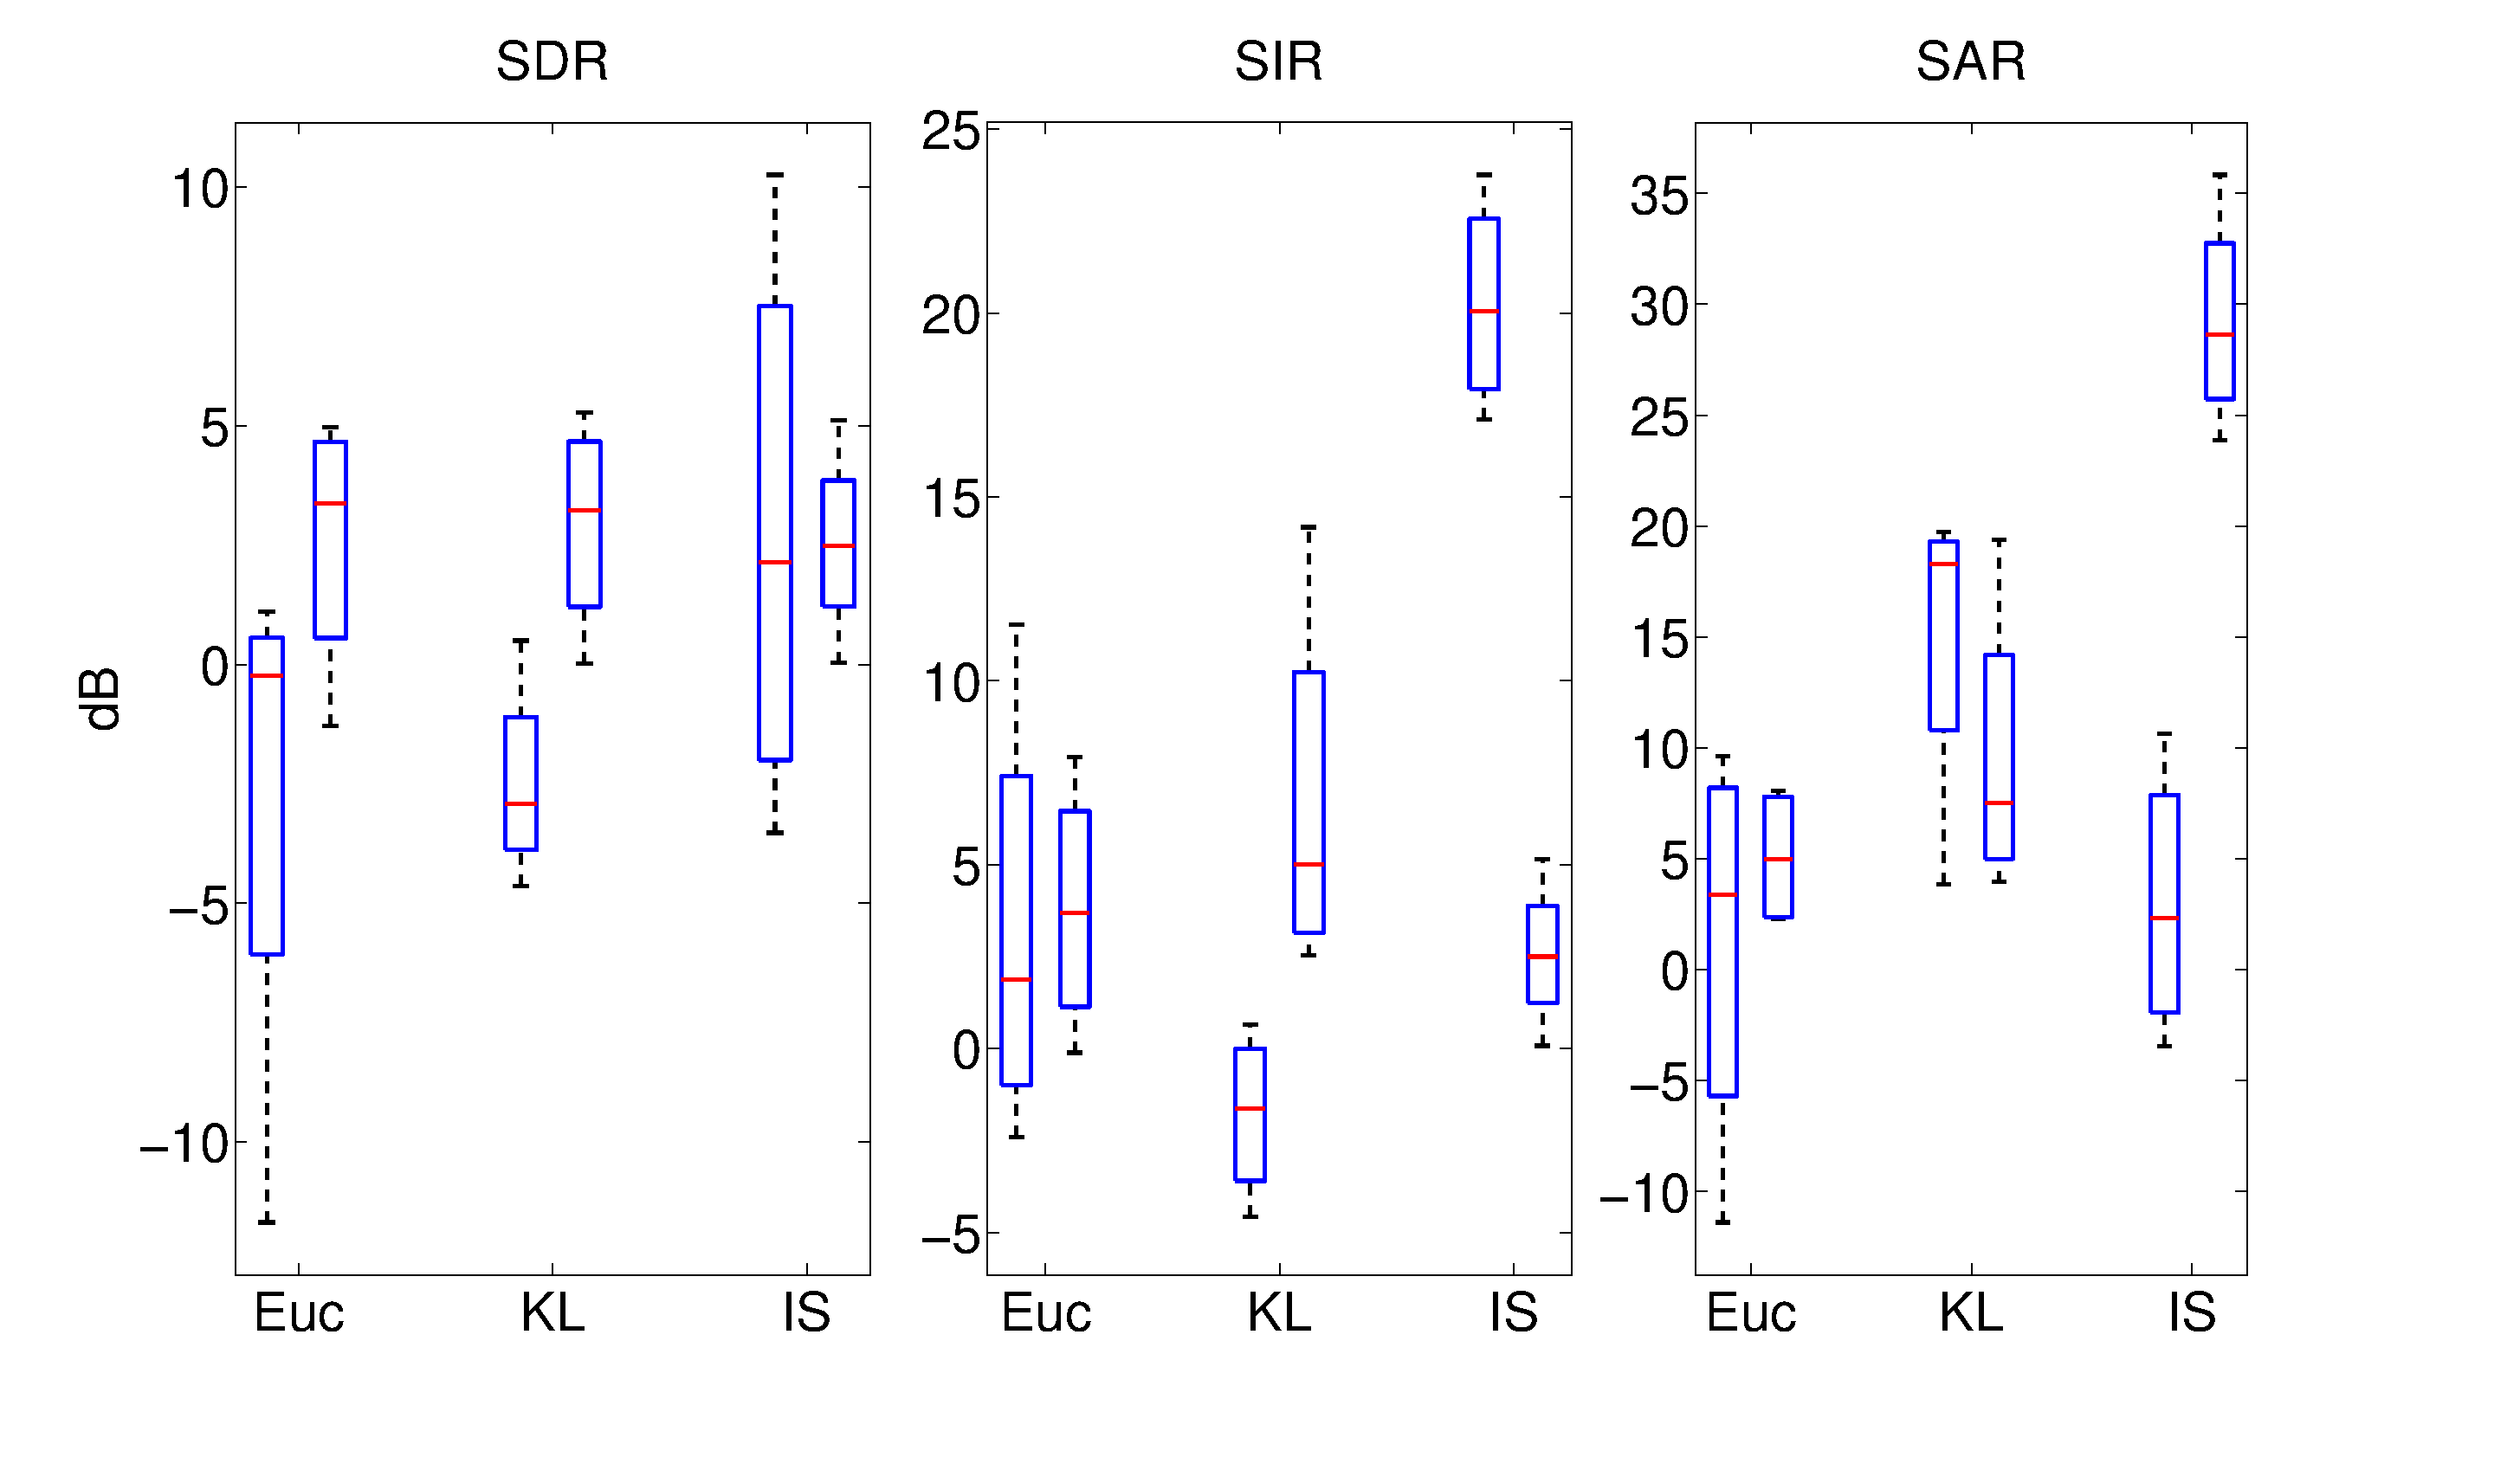
\includegraphics[width=9cm]{fig/NewDictDivTest}
%  \vspace{2.0cm}
  \caption{\label{frame2048} SDR, SIR and SAR of harmonic (left bar)/percussive (right bar) estimated sources on the SiSec database with a window frame of $2048$ samples.}
  
\end{figure}



\subsection{Influence of the dictionary}
\label{setup:dictionary}

%We now discuss the influence of the dictionary. We compare the two methods described in Section~\ref{fixedict}. In addition to that, we test a third dictionary is made by the concatenation of the first two dictionaries. The more information contained in the dictionary, the likely the decomposition to properly extract the percussive part. On some signals, the algorithm is not able to extract a lot of energy from the mixture as no atom from the dictionary correspond to any of the percussive signal.
%We display on Figure~\ref{resultsDict} the SDR results of the decomposition using the NMF dictionary, the STFT dictionary as well as the concatenated dictionary. The SAR and SIR are postponed in Appendix~\ref{appendix:dict} on Figures~\ref{resultsDictSAR} and~\ref{resultsDictSIR} respectively. In our tests, the results with the concatenated dictionary give the highest score. Indeed, the concatenated dictionary contains the largest amount of information and as a result, obtains the best separation. As the dictionary is fixed, it is important to have a large dictionary to be able to extract a large type of percussive instruments. The STFT and the NMF dictionaries give results similar to each other. The two dictionaries contain complementary information that allow for a better separation while they are concatenated. In the tests we will conduct later in Section~\ref{sec:stateoftheart} on a large database, we will use the concatenated dictionary as it contains the largest amount of information. 

We now discuss the different methods to construct the drum dictionary. As the dictionary is fixed, it is important to find a good compromise with the size and the quantity of information contained. 
Two types of audio recordings are available, the first type contains drum hits of the independents element of the drum kit. We concatenated the recording of the drum hits of each drummer in three $10$~min long audio signals. The other type of audio files are drum phrases. We created three signals of different length ($6$~min, $12$~min, $30$~min) for the three drummers for a total of $9$ audio signal. 
Finally, we compute the STFT of these $12$ signals and we execute a NMF on each of the spectrograms to obtain various dictionaries. The rank of the decomposition is chosen as $k \in [6,9,12,25,50,100,200,500]$. In total, $108$ dictionaries are created. 

Multiple tests are run in order to evaluate the influence of each of the parameters for the training step. The drum kit of each drummer are very different and they provide different information for the decomposition. We display on Figure~\ref{resultsDict} the mean SDR, SIR and SAR results of the average results for each drummer. Figure \ref{resultsDict} shows that the information of the drummer $2$ is the most relevant for our test. The drummer $1$ plays on a very small drum kit that does not contains enough information. Finally the drummer $3$ plays uses a large drumset with many elements that are not usually present in most recording and because of that the dictionary is too diverse.

Now the rest of the experiment are conducted using the dictionaries constructed on the audio files from drummer $2$. Figure \ref{resultsDictLength} show the influence of the length of the training data on the results. Above $6$~min of training data, the quality of the decomposition decreases so in the rest of the experiment, we used the dictionaries computed of these data.

Finally, Figure \ref{resultsDictD2} show the results wrt the rank of factorization. The best results are obtained for $k=12$. Bellow that, the dictionary is too small and not enough information is captured. Inversely, if the rank is chosen too big during the learning process, the dictionary does not capture the percussive part satisfyingly during the decomposition.

For the rest of the article, we will use a dictionary constructed using a $6$~min long audio signal from the drummer $2$ with $k=12$.

\begin{figure}[t]

  \centering 
  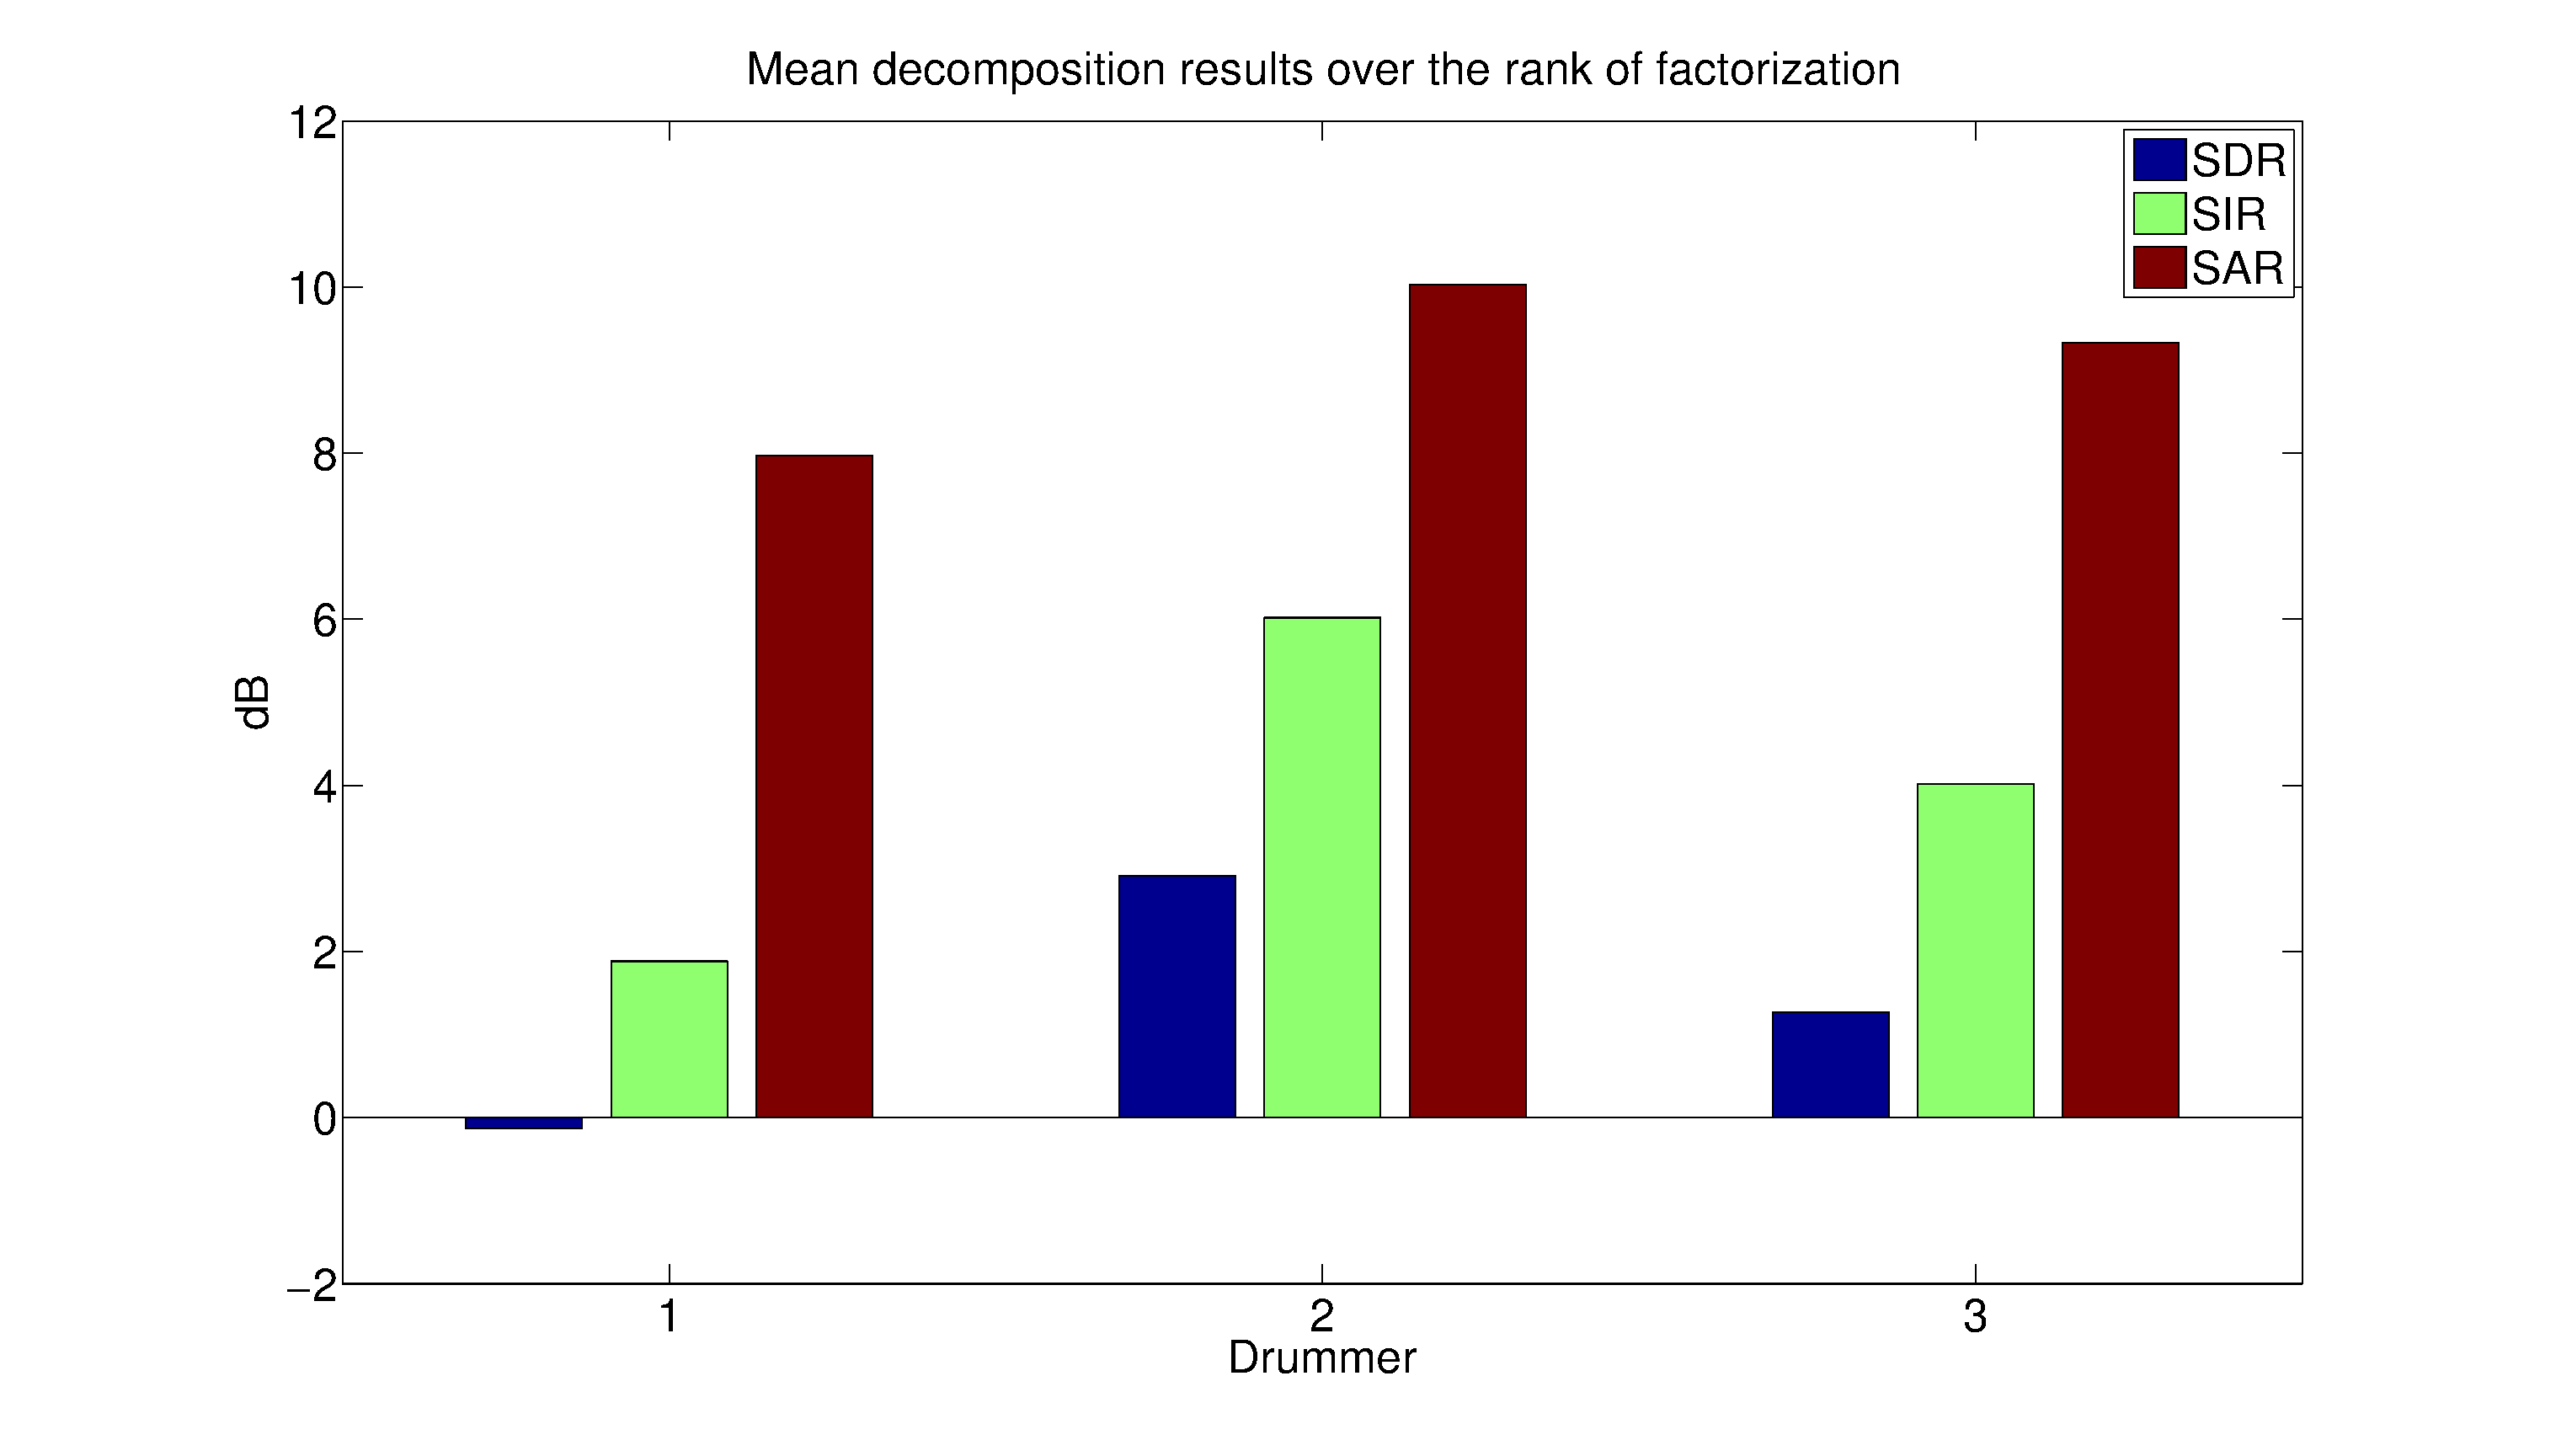
\includegraphics[width=8cm]{fig/ResultsMeanRank}
%  \vspace{2.0cm}
  \caption{\label{resultsDict} Mean SDR SIR and SAR results averaged for each drummer on the SiSec database.}
  
\end{figure}

\begin{figure}[t]

  \centering 
  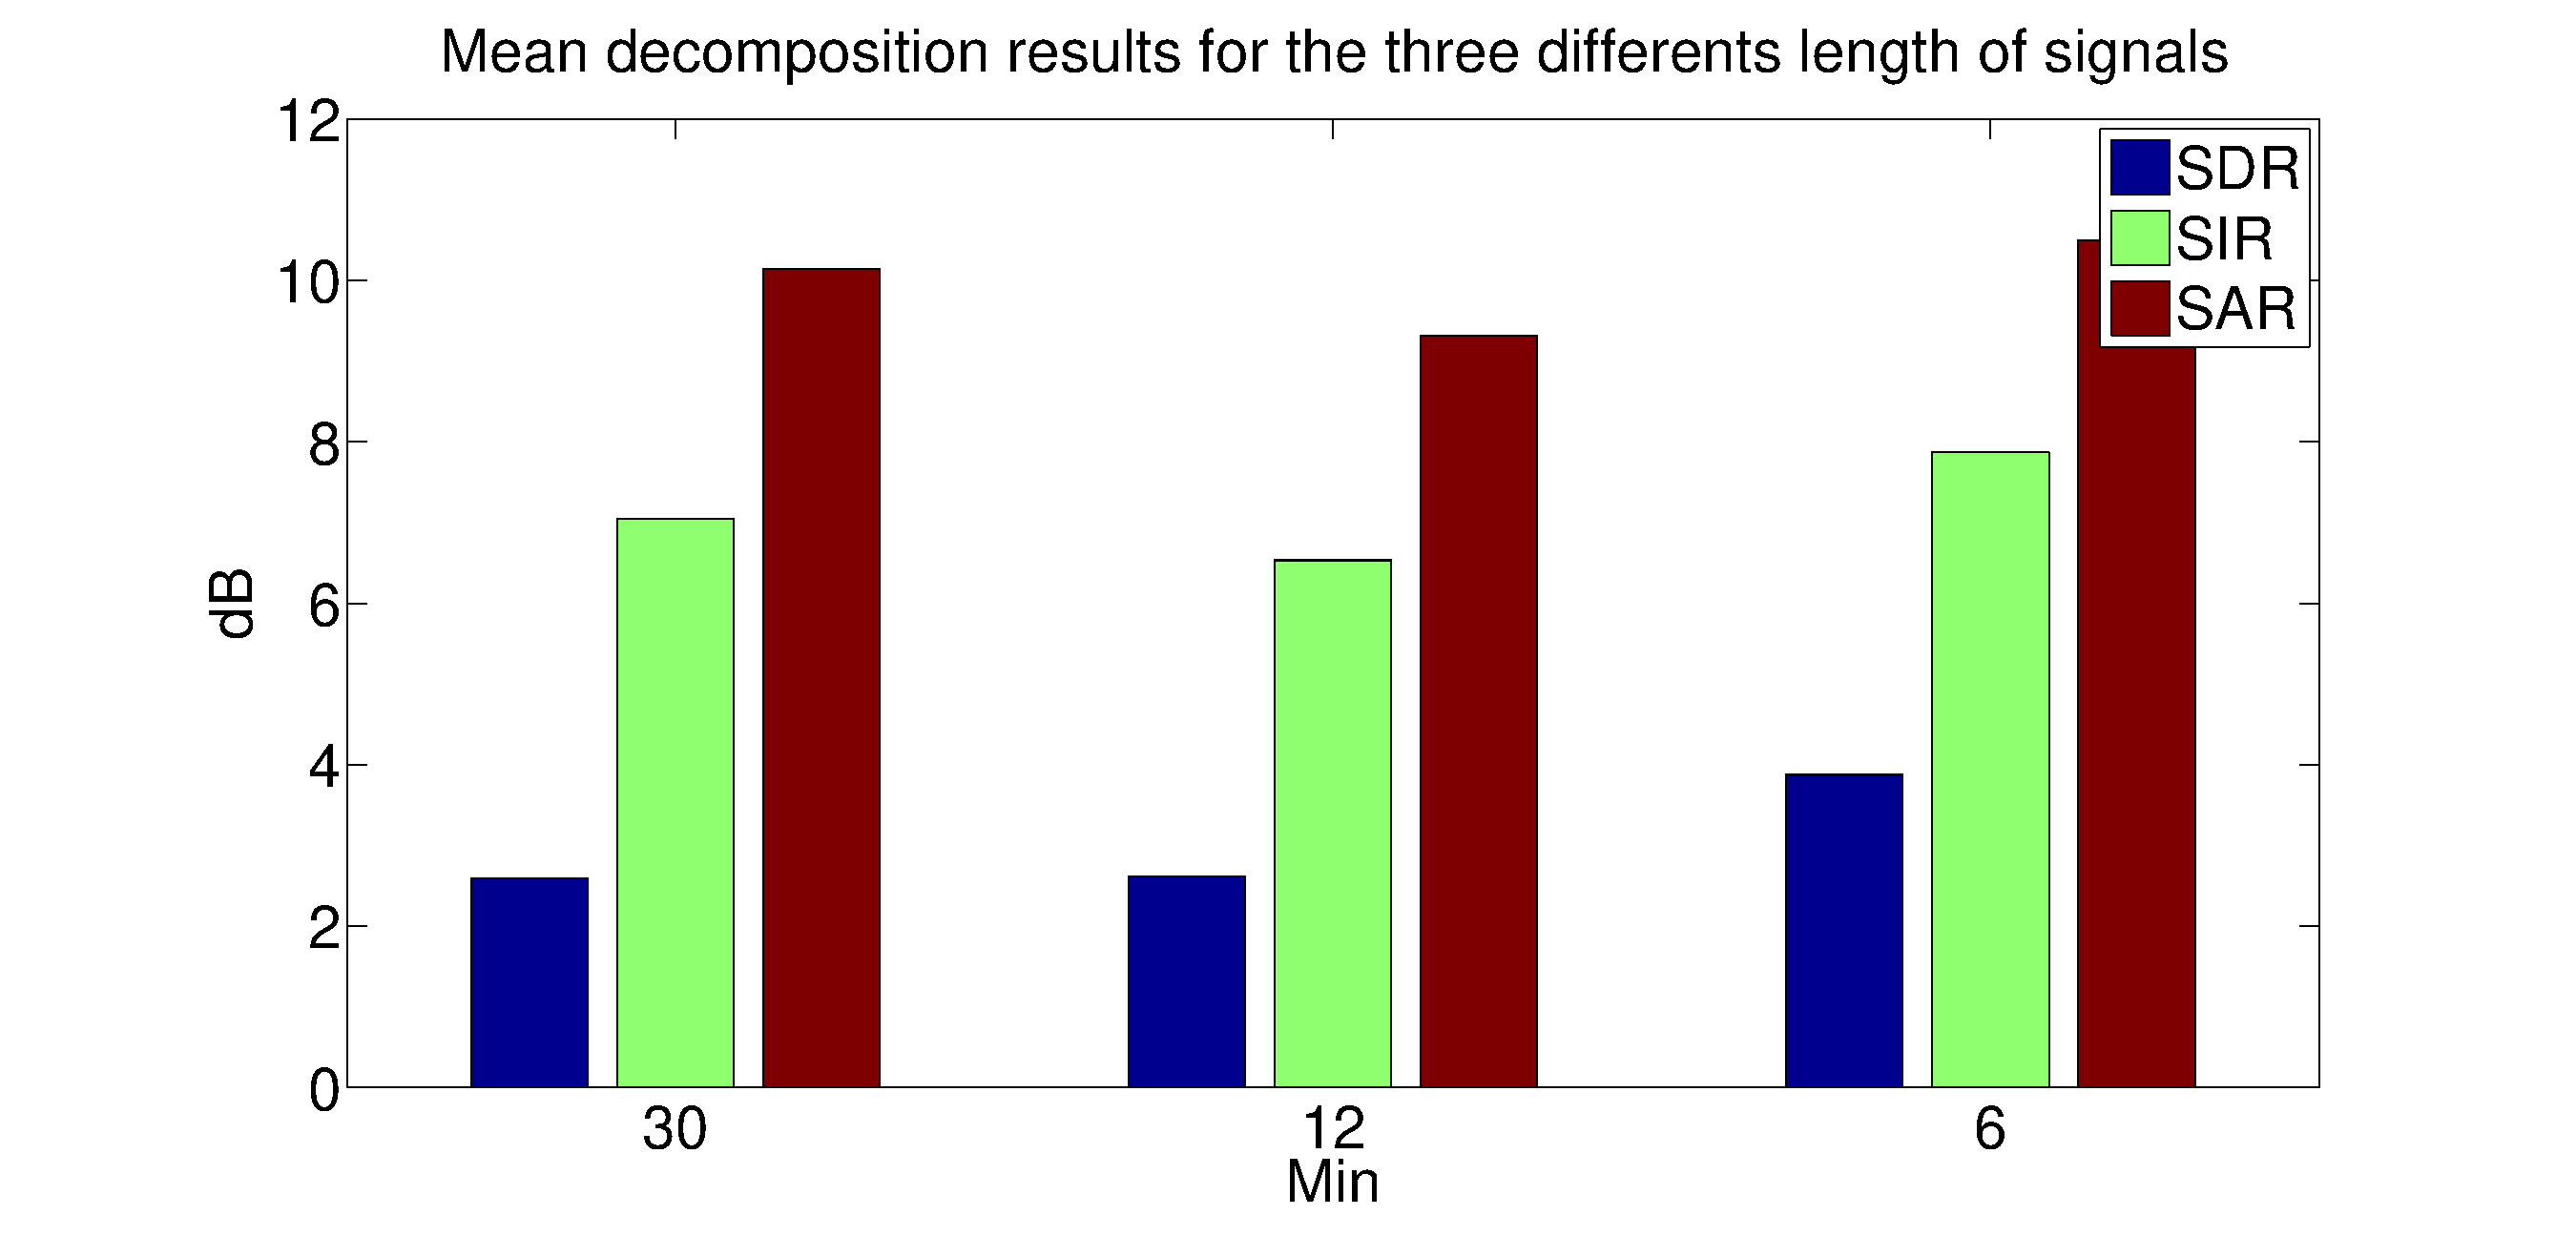
\includegraphics[width=8cm]{fig/ResultsMeanLength}
%  \vspace{2.0cm}
  \caption{\label{resultsDictLength} Mean SDR SIR and SAR results for the dictionaries learned with different signal length on the SiSec database.}
  
\end{figure}
\begin{figure}[t]

  \centering 
  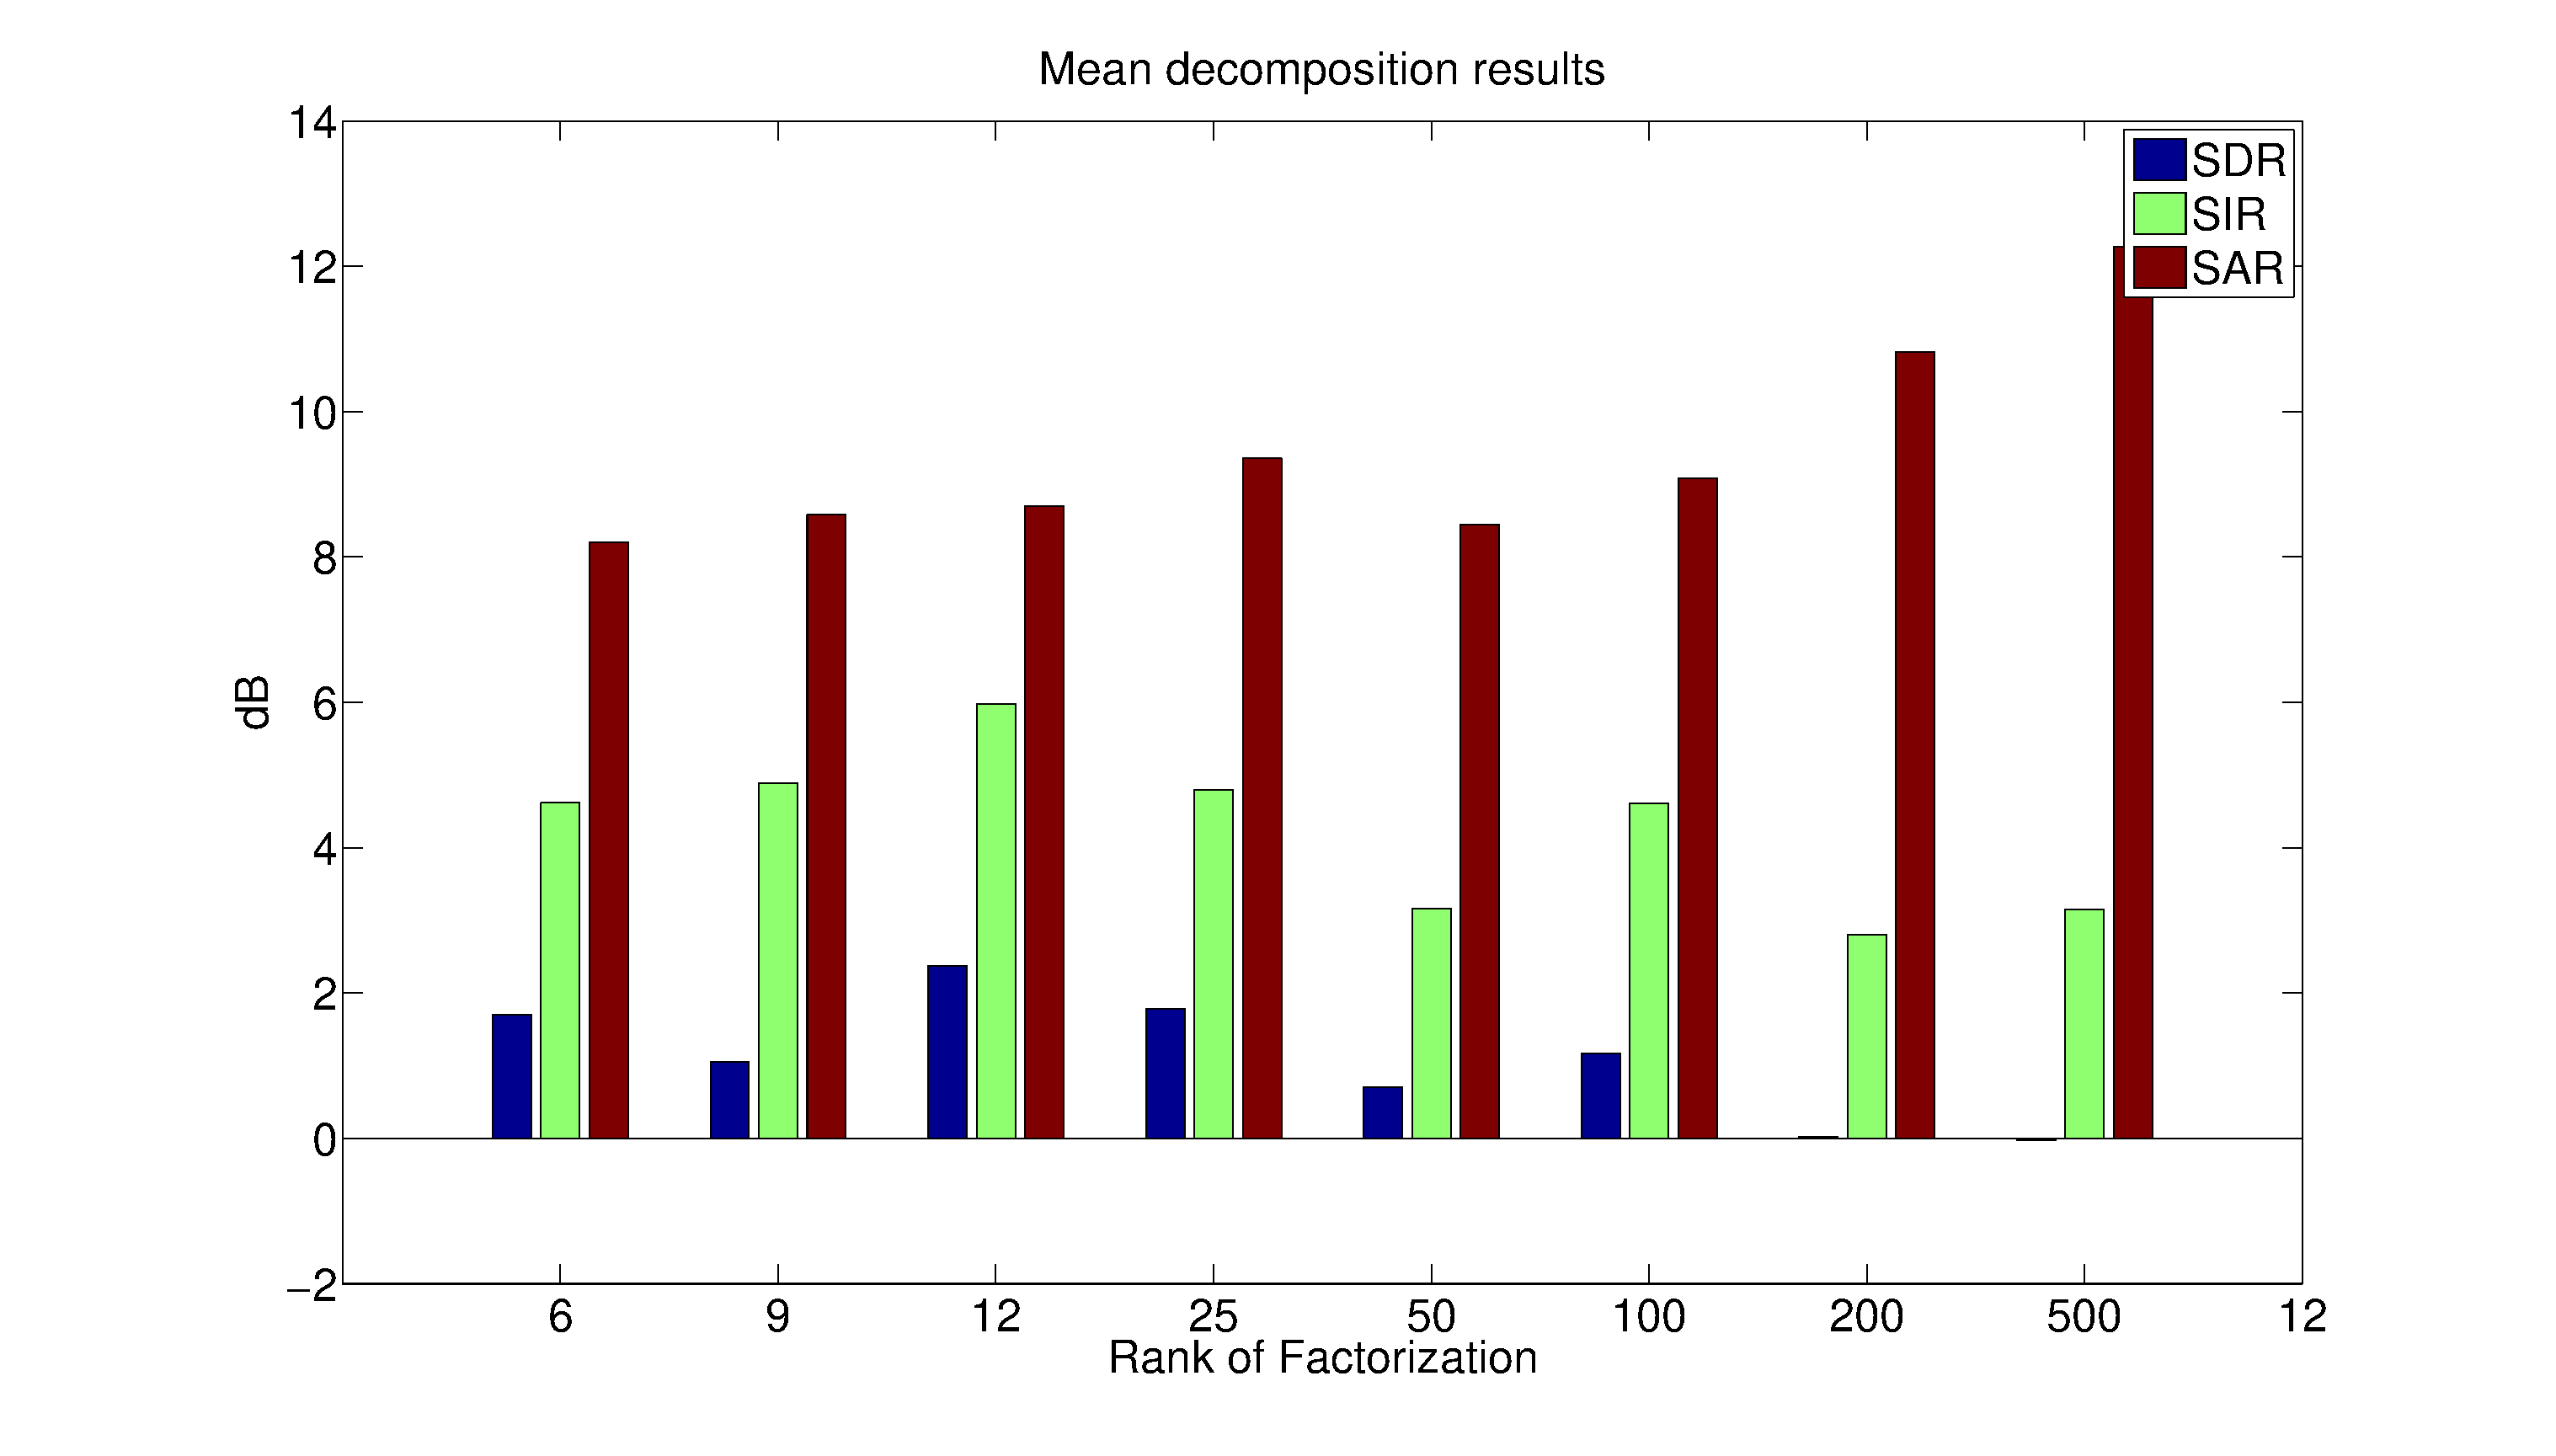
\includegraphics[width=8cm]{fig/ResultsDictDrummer2}
%  \vspace{2.0cm}
  \caption{\label{resultsDictD2} Mean SDR SIR and SAR results for various rank of factorization on the SiSec database.}
  
\end{figure}



